\documentclass[border=10pt]{standalone}
\usepackage[svgnames]{xcolor}
\usepackage{amsmath}
\usepackage{pgfplots}
\pgfplotsset{compat=newest}
\usepackage[sfdefault]{FiraSans}
\usepackage{FiraMono}
\renewcommand*\familydefault{\sfdefault}
\begin{document}
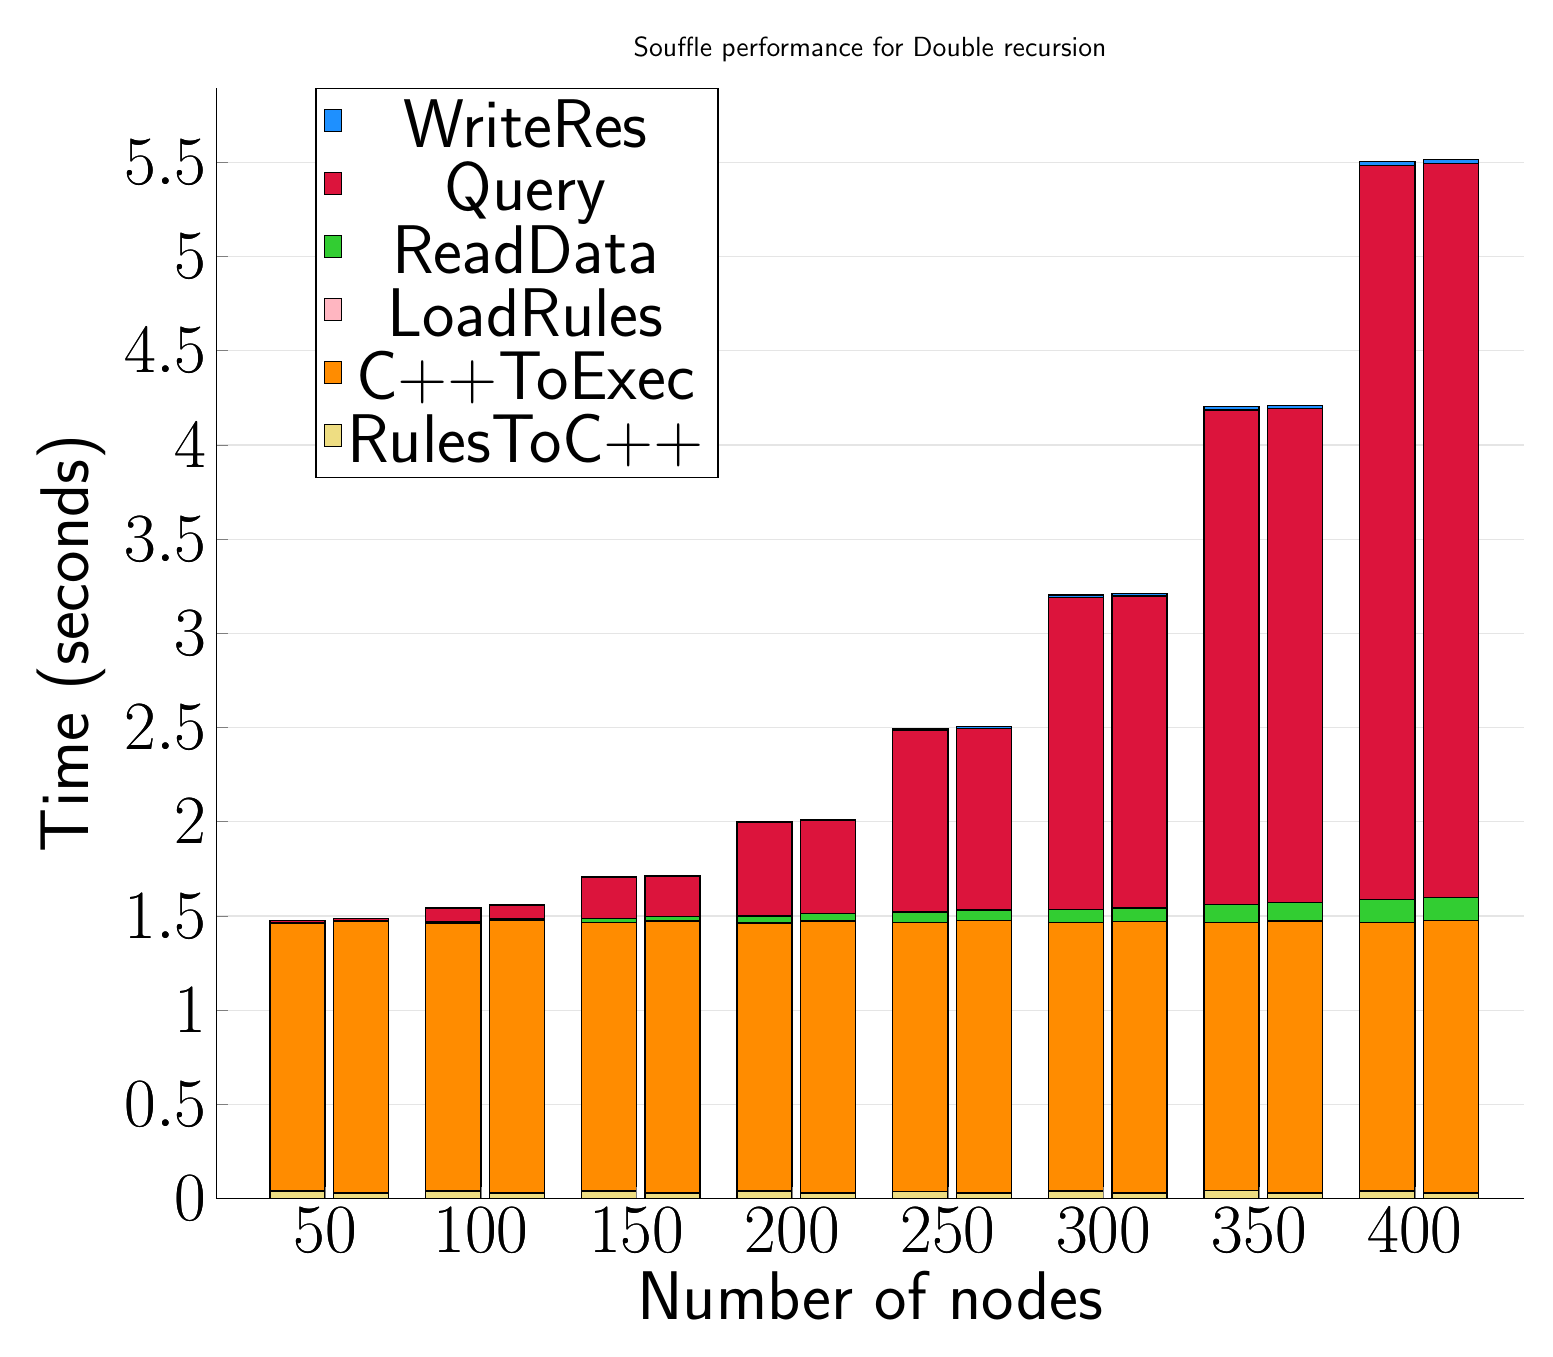
\begin{tikzpicture}
\begin{axis}[
   ybar stacked,
   title={Souffle performance for Double recursion},
   bar shift=-10pt,
   width=1.5\textwidth,
   bar width=0.7cm,
   ymajorgrids, tick align=inside,
   major grid style={draw=gray!20},
   xtick=data,
   ymin=0, ymax=5.895328,
   axis x line*=bottom,
   axis y line*=left,
   enlarge x limits=0.1,
   legend style={
       at={(0.23, 1)},
       anchor=north,
       legend columns=1,
       font=\Huge,
   },
   ylabel={Time (seconds)},
   xlabel={Number of nodes},
   label style={font=\Huge},
   tick label style={font=\Huge},
]
\addlegendimage{fill=DodgerBlue, draw=black, line width=0.2pt}
\addlegendentry{WriteRes}
\addlegendimage{fill=Crimson, draw=black, line width=0.2pt}
\addlegendentry{Query}
\addlegendimage{fill=LimeGreen, draw=black, line width=0.2pt}
\addlegendentry{ReadData}
\addlegendimage{fill=LightPink, draw=black, line width=0.2pt}
\addlegendentry{LoadRules}
\addlegendimage{fill=DarkOrange, draw=black, line width=0.2pt}
\addlegendentry{C++ToExec}
\addlegendimage{fill=LightGoldenrod, draw=black, line width=0.2pt}
\addlegendentry{RulesToC++}
\addplot +[fill=LightGoldenrod, draw=black, line width=0.5pt] coordinates {
    (50, 0.040000081062316895)
    (100, 0.039999985694885255)
    (150, 0.040999984741210936)
    (200, 0.040999984741210936)
    (250, 0.03900001049041748)
    (300, 0.039999985694885255)
    (350, 0.04199995994567871)
    (400, 0.04100003242492676)
};
\addplot +[fill=DarkOrange, draw=black, line width=0.5pt] coordinates {
    (50, 1.4209999561309814)
    (100, 1.4230000019073485)
    (150, 1.4230000019073485)
    (200, 1.4210000038146973)
    (250, 1.4269999742507935)
    (300, 1.4240000247955322)
    (350, 1.4230000019073485)
    (400, 1.4229999780654907)
};
\addplot +[fill=LightPink, draw=black, line width=0.5pt] coordinates {
    (50, 0.00012074989999999999)
    (100, 6.26875e-05)
    (150, 0.0001261123)
    (200, 0.00012127079999999998)
    (250, 0.0001228627)
    (300, 9.689590000000001e-05)
    (350, 0.00010978350000000001)
    (400, 0.00012832099999999998)
};
\addplot +[fill=LimeGreen, draw=black, line width=0.5pt] coordinates {
    (50, 0.002824354)
    (100, 0.008827278000000001)
    (150, 0.02226669)
    (200, 0.037610309999999994)
    (250, 0.05466174)
    (300, 0.07163775)
    (350, 0.09631645)
    (400, 0.12345740000000001)
};
\addplot +[fill=Crimson, draw=black, line width=0.5pt] coordinates {
    (50, 0.01265763)
    (100, 0.06916994000000001)
    (150, 0.21619569999999996)
    (200, 0.4962427)
    (250, 0.9655375000000002)
    (300, 1.65581)
    (350, 2.624407)
    (400, 3.895328)
};
\addplot +[fill=DodgerBlue, draw=black, line width=0.5pt] coordinates {
    (50, 0.0006516165)
    (100, 0.001722833)
    (150, 0.003756075)
    (200, 0.005688709)
    (250, 0.009238070999999997)
    (300, 0.012716830000000002)
    (350, 0.01719419)
    (400, 0.02239635)
};
\end{axis}
\begin{axis}[
   ybar stacked,
   bar shift=13pt,
   width=1.5\textwidth,
   bar width=0.7cm,
   ymajorgrids, tick align=inside,
   major grid style={draw=none},
   xtick=data,
   ymin=0, ymax=5.895328,
   axis x line*=none,
   axis y line*=none,
   enlarge x limits=0.1,
   label style={font=\Huge},
   tick label style={font=\Huge},
]
\addplot +[fill=LightGoldenrod, draw=black, line width=0.5pt] coordinates {
    (50, 0.030000000000000006)
    (100, 0.030000000000000006)
    (150, 0.030000000000000006)
    (200, 0.030000000000000006)
    (250, 0.030000000000000006)
    (300, 0.030000000000000006)
    (350, 0.030000000000000006)
    (400, 0.030000000000000006)
};
\addplot +[fill=DarkOrange, draw=black, line width=0.5pt] coordinates {
    (50, 1.4409999999999996)
    (100, 1.448)
    (150, 1.444)
    (200, 1.4439999999999997)
    (250, 1.4459999999999997)
    (300, 1.4409999999999998)
    (350, 1.4439999999999995)
    (400, 1.4449999999999996)
};
\addplot +[fill=LightPink, draw=black, line width=0.5pt] coordinates {
    (50, 0.0001197)
    (100, 6.23e-05)
    (150, 0.000125)
    (200, 0.00012030000000000001)
    (250, 0.00012169999999999998)
    (300, 9.620000000000001e-05)
    (350, 0.00010890000000000002)
    (400, 0.0001275)
};
\addplot +[fill=LimeGreen, draw=black, line width=0.5pt] coordinates {
    (50, 0.0028233)
    (100, 0.0088252)
    (150, 0.022247499999999996)
    (200, 0.037603399999999995)
    (250, 0.0546508)
    (300, 0.07162400000000001)
    (350, 0.09626309999999999)
    (400, 0.12342810000000001)
};
\addplot +[fill=Crimson, draw=black, line width=0.5pt] coordinates {
    (50, 0.0126552)
    (100, 0.06914200000000001)
    (150, 0.21575950000000002)
    (200, 0.4960197)
    (250, 0.9646997)
    (300, 1.6551380000000002)
    (350, 2.623153)
    (400, 3.8939400000000006)
};
\addplot +[fill=DodgerBlue, draw=black, line width=0.5pt] coordinates {
    (50, 0.000651)
    (100, 0.0014976999999999998)
    (150, 0.0032937)
    (200, 0.0056438)
    (250, 0.008795500000000001)
    (300, 0.012630800000000001)
    (350, 0.0170334)
    (400, 0.0221109)
};
\end{axis}
\end{tikzpicture}

\end{document}
